
\section{椭圆的极点极线初探}
\label{sec:oval-pole-line}

椭圆曲线将其所在平面分成了三个部分:椭圆内部、椭圆曲线上、椭圆外部,对于椭圆曲线上的点,正如大家所熟知的,它们的坐标都满足椭圆的方程:
\begin{equation}
\frac{x^2}{a^2}+\frac{y^2}{b^2}=1 \label{eq:ellipse}
\end{equation}
而对于椭圆内部的点,它们的坐标都满足不等式:
\begin{equation}
\frac{x^2}{a^2}+\frac{y^2}{b^2}<1 \label{neq:innerellipse}
\end{equation}
这个很好理解,对于椭圆内部任何一点,总能在椭圆上找到一个对应点,使其横坐标相同而纵坐标的绝对值大于椭圆内的点,而椭圆曲线上的这个对应点的坐标满足方程\ref{eq:ellipse},那么椭圆内的点的坐标满足不等式\ref{neq:innerellipse}就是显然的事情了。
至于椭圆外部的点,那就只有成立不等式:
\begin{equation}
\frac{x^2}{a^2}+\frac{y^2}{b^2}>1 \label{neq:outerellipse}
\end{equation}
因为之前椭圆曲线与其方程之间以及椭圆内部的平面区域与其不等式之间都是可以互推的。

接下来讨论椭圆的切线问题,在椭圆上任取一个点 $P(x_0,y_0)$,那么该点处的切线方程将是:
\begin{equation}
\frac{x_0x}{a^2}+\frac{y_0y}{b^2}=1 \label{eq:tangent}
\end{equation}
\begin{center}
%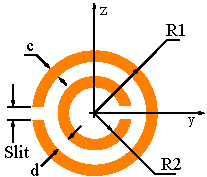
\includegraphics{fig1.png}
\end{center}
这直线为何就是切线方程呢?在这直线上任取一点 $T(x_T,y_T)$,有:
\begin{equation}
(\frac{x_0^2}{a^2}+\frac{y_0^2}{b^2})+(\frac{x_T^2}{a^2}+\frac{y_T^2}{b^2}) \geqslant 2(\frac{x_0x_T}{a^2}+\frac{y_0y_T}{b^2})=2
\end{equation}
所以得到:
\begin{equation}
\frac{x_T^2}{a^2}+\frac{y_T^2}{b^2} \geqslant 1
\end{equation}
这表明直线\ref{eq:tangent}上除点$P$外任何一点都在椭圆外,与椭圆只有$P$一个交点,所以它理所当然就是点$P$处的切线方程。

现在在椭圆外任选一个点 $P(x_0,y_0)$,并由它向椭圆引两条切线,切点分别为 $T_1(x_1,y_1)$和$T_2(x_2,y_2)$,由于点$P$同时在两条切线上,所以同时成立着:
\begin{equation}
\frac{x_0 x_1}{a^2}+\frac{y_0 y_1}{b^2} = 1,\frac{x_0 x_2}{a^2}+\frac{y_0 y_2}{b^2} = 1
\end{equation}
由此立刻得知切点弦 $T_1 T_2$ 的方程是:
\begin{equation}
\frac{x_0x}{a^2}+\frac{y_0y}{b^2}=1   \label{eq:qiedianxian}
\end{equation}
这一点令人惊讶,要注意这时点$P$是在椭圆外,所以不要与刚才所证的切线方程混淆了。同样的方程,因为点$P$位置的不同,它代表的直线也不同。相信读者此时也会不失时机的提出如下问题:如果点$P$是在椭圆内部,那么方程\ref{eq:qiedianxian}又代表什么样的直线呢?此刻还不好回答,但后文自然而然的会得出结论。

接着讨论弦的中点的问题,在椭圆上任取两点 $T_1(x_1,y_1)$和$T_2(x_2,y_2)$,线段$T_1T_2$中点为$Q(x_Q,y_Q)$,那么首先成立着等式:
\begin{equation}
\frac{x_1^2}{a^2}+\frac{y_1^2}{b^2}=1, \frac{x_2^2}{a^2}+\frac{y_2^2}{b^2}=1
\end{equation}
两式相减得到:
\begin{equation}
\frac{x_1^2-x_2^2}{a^2}+\frac{y_1^2-y_2^2}{b^2}=0
\end{equation}
进一步变形为:
\begin{equation}
\frac{y_1-y_2}{x_1-x_2}\frac{\frac{y_1+y_2}{2}}{\frac{x_1+x_2}{2}}=-\frac{b^2}{a^2}
\end{equation}
所以弦$T_1T_2$及中点与椭圆中心连线$OQ$两者斜率之积为定值\footnote{本文中都不考虑斜率不存在等特殊情况,只就一般性的情况进行叙述,以得出一般性的结论。}:
\begin{equation}
k_{T_1T_2}k_{OQ}=-\frac{b^2}{a^2}
\end{equation}
据此可以知道若另作一弦使其所在直线平行于$OQ$,那么其中点与椭圆中心的连线必平行于直线$T_1T_2$,即两个方向存在着相互性,这称之为椭圆的一组“共轭方向”,而这个结论则可以视为椭圆中的垂径定理。此外还可以知道,对于椭圆内部任何一个点,在经过它的所有弦中,只有唯一一条能使它成为弦的中点,而该弦的方向,就是该点与椭圆中心连线的共轭方向。而如果在这里平行移动弦$T_1T_2$,直到它成为椭圆的切线$l$,假如切点为$P(x_0,y_0)$,那么我们应该得出:
\begin{equation}
k_l k_{OP}=-\frac{b^2}{a^2}
\end{equation}
这与我们刚才所推导的点$P$处的切线方程正好吻合。

回到刚才过椭圆外一点$P(x_0,y_0)$引两条切线$PT_1$及$PT_2$的场景中,以$Q$标记切点弦$T_1T_2$的中点,则点$Q$的坐标必然满足切点弦$T_1T_2$的方程:
\begin{equation}
\frac{x_0 x_Q}{a^2}+\frac{y_0 y_Q}{b^2} = 1 \label{eq:pq}
\end{equation}
这一点就很有意思了,因为这意味着点$P$位于下面的直线上:
\begin{equation}
\frac{x_Q x}{a^2}+\frac{y_Q y}{b^2} = 1 \label{abc}
\end{equation}
这是一条什么样的直线呢?容易发现,它的方向就是$OQ$的共轭方向!现在回想一下前面所提的悬而未决的问题:对于椭圆内的一点,方程\ref{eq:qiedianxian}代表什么样的直线,现在就可以理直气壮的回答说,先找出以椭圆内的这点为中点的弦,然后过此弦两端点引椭圆切线,两切线有一个交点,
这条直线就经过了这个点,那么方向呢?将椭圆内的这点与椭圆中心相连,其共轭方向就是该直线的方向!这段长长的描述显得有些不符合数学美感,但至少我们解决了如下问题:针对椭圆上、椭圆内、椭圆外的点$P(x_0,y_0)$,方程\ref{eq:qiedianxian}各自分别代表什么样的直线,而且还可以知道,椭圆内(除去中心)与椭圆外的点之间,存在着一种对称关系,借此我们可以在这两大平面区域之间,建立一对一的映射关系。

进一步,直线$OQ$与$T_1T_2$是共轭的,而现在直线\ref{abc}的方向也与$OQ$共轭,这表明直线\ref{abc}与切点弦$T_1T_2$是平行的!比较一下方程\ref{abc}与方程
\ref{eq:qiedianxian}就可以得出结论:直线$PQ$是经过椭圆中心的!进而记$R$为线段$PQ$与椭圆的交点,那么显然:
\begin{equation}
\frac{x_R^2}{a^2}+\frac{y_R^2}{b^2}=1 \label{eq:r}
\end{equation}
比较一下方程\ref{eq:pq}与\ref{eq:r},再加之我们知道$P$、$Q$、$R$三点共线,而且还过椭圆中心,所以:
\begin{equation}
x_0 x_Q=x_R^2,y_0 y_Q=y_R^2
\end{equation}
由此得到:
\begin{equation}
OP\cdot OQ = OR^2
\end{equation}
一切都是如此的完美。

前面曾经考虑过,当点$P(x_0,y_0)$在椭圆内部时,方程\ref{eq:tangent}所代表的直线似乎难以描述,现在我们给它取一个好听的名字:极线。准确的说,是点$P$ 关于该椭圆的极线,而点$P$则称为直线\ref{eq:tangent}关于椭圆的极点。当点$P$在椭圆曲线上时,它关于椭圆的极线就是椭圆在该点处的切线(相切),当点$P$在椭圆外部时,它关于椭圆的极线就是对应的切点弦所在直线(相交),而当点$P$在椭圆内时,对应的极线就在椭圆外部了(相离)。而且我们看到,点$P$无论位于哪个位置(椭圆中心除外),它关于椭圆的极线的方向都是$OP$ 的共轭方向,所以如果让点$P$在一条从椭圆中心出发的射线上由椭圆内到椭圆外缓慢移动,我们将看到它关于椭圆的极线由远及近平行移动,当点$P$ 移到椭圆上的那一刻,极点刚好位于极线上,而极线也成为过极点的切线,此后,当点$P$移动到椭圆外时,极线则与椭圆椭圆相交,当点$P$向无穷远处移动时,极线则向椭圆中心无限靠近。容易看出,对于平面上任何一点(椭圆中心除外),它关于椭圆的极线都是唯一存在的,反过来,对于平面上任何一条不通过椭圆中心的直线,它关于椭圆的极点也是唯一存在的。而切点与切线,不过是极点刚好位于极线上的一种特殊情况罢了。

